\documentclass[letterpaper]{article}
%\documentclass[a5paper]{article}

%% Language and font encodings
\usepackage[english]{babel}
\usepackage[utf8x]{inputenc}
\usepackage[T1]{fontenc}

%% Sets page size and margins
\usepackage[letterpaper,top=1in,bottom=1in,left=1in,right=1in,marginparwidth=1.75cm]{geometry}
%\usepackage[a5paper,top=1cm,bottom=1cm,left=1cm,right=1.5cm,marginparwidth=1.75cm]{geometry}

\usepackage{graphicx}
\graphicspath{ {./} }	  %%where to look for images

%% Useful packages
\usepackage{amssymb, amsmath, amsthm} 
%\usepackage{graphicx}  %%this is currently enabled in the default document, so it is commented out here. 
\usepackage{calrsfs}
\usepackage{braket}
\usepackage{mathtools}
\usepackage{lipsum}
\usepackage{tikz}
\usetikzlibrary{cd}
\usepackage{verbatim}
%\usepackage{ntheorem}% for theorem-like environments
\usepackage{mdframed}%can make highlighted boxes of text
%Use case: https://tex.stackexchange.com/questions/46828/how-to-highlight-important-parts-with-a-gray-background
\usepackage{wrapfig}
\usepackage{centernot}
\usepackage{subcaption}%\begin{subfigure}{0.5\textwidth}
\usepackage{pgfplots}
\pgfplotsset{compat=1.13}
\usepackage[colorinlistoftodos]{todonotes}
\usepackage[colorlinks=true, allcolors=blue]{hyperref}
\usepackage{xfrac}					%to make slanted fractions \sfrac{numerator}{denominator}
\usepackage{enumitem}            
    %syntax: \begin{enumerate}[label=(\alph*)]
    %possible arguments: f \alph*, \Alph*, \arabic*, \roman* and \Roman*
\usetikzlibrary{arrows,shapes.geometric,fit}

\DeclareMathAlphabet{\pazocal}{OMS}{zplm}{m}{n}
%% Use \pazocal{letter} to typeset a letter in the other kind 
%%  of math calligraphic font. 

%% This puts the QED block at the end of each proof, the way I like it. 
\renewenvironment{proof}{{\bfseries Proof}}{\qed}
\makeatletter
\renewenvironment{proof}[1][\bfseries \proofname]{\par
  \pushQED{\qed}%
  \normalfont \topsep6\p@\@plus6\p@\relax
  \trivlist
  %\itemindent\normalparindent
  \item[\hskip\labelsep
        \scshape
    #1\@addpunct{}]\ignorespaces
}{%
  \popQED\endtrivlist\@endpefalse
}
\makeatother

%% This adds a \rewnewtheorem command, which enables me to override the settings for theorems contained in this document.
\makeatletter
\def\renewtheorem#1{%
  \expandafter\let\csname#1\endcsname\relax
  \expandafter\let\csname c@#1\endcsname\relax
  \gdef\renewtheorem@envname{#1}
  \renewtheorem@secpar
}
\def\renewtheorem@secpar{\@ifnextchar[{\renewtheorem@numberedlike}{\renewtheorem@nonumberedlike}}
\def\renewtheorem@numberedlike[#1]#2{\newtheorem{\renewtheorem@envname}[#1]{#2}}
\def\renewtheorem@nonumberedlike#1{  
\def\renewtheorem@caption{#1}
\edef\renewtheorem@nowithin{\noexpand\newtheorem{\renewtheorem@envname}{\renewtheorem@caption}}
\renewtheorem@thirdpar
}
\def\renewtheorem@thirdpar{\@ifnextchar[{\renewtheorem@within}{\renewtheorem@nowithin}}
\def\renewtheorem@within[#1]{\renewtheorem@nowithin[#1]}
\makeatother

%% This makes theorems and definitions with names show up in bold, the way I like it. 
\makeatletter
\def\th@plain{%
  \thm@notefont{}% same as heading font
  \itshape % body font
}
\def\th@definition{%
  \thm@notefont{}% same as heading font
  \normalfont % body font
}
\makeatother

%===============================================
%==============Shortcut Commands================
%===============================================
\newcommand{\ds}{\displaystyle}
\newcommand{\B}{\mathcal{B}}
\newcommand{\C}{\mathbb{C}}
\newcommand{\F}{\mathbb{F}}
\newcommand{\N}{\mathbb{N}}
\newcommand{\R}{\mathbb{R}}
\newcommand{\Q}{\mathbb{Q}}
\newcommand{\T}{\mathcal{T}}
\newcommand{\Z}{\mathbb{Z}}
\renewcommand\qedsymbol{$\blacksquare$}
\newcommand{\qedwhite}{\hfill\ensuremath{\square}}
\newcommand*\conj[1]{\overline{#1}}
\newcommand*\closure[1]{\overline{#1}}
\newcommand*\mean[1]{\overline{#1}}
%\newcommand{\inner}[1]{\left< #1 \right>}
\newcommand{\inner}[2]{\left< #1, #2 \right>}
\newcommand{\powerset}[1]{\pazocal{P}(#1)}
%% Use \pazocal{letter} to typeset a letter in the other kind 
%%  of math calligraphic font. 
\newcommand{\cardinality}[1]{\left| #1 \right|}
\newcommand{\domain}[1]{\mathcal{D}(#1)}
\newcommand{\image}{\text{Im}}
\newcommand{\inv}[1]{#1^{-1}}
\newcommand{\preimage}[2]{#1^{-1}\left(#2\right)}
\newcommand{\script}[1]{\mathcal{#1}}


\newenvironment{highlight}{\begin{mdframed}[backgroundcolor=gray!20]}{\end{mdframed}}

\DeclarePairedDelimiter\ceil{\lceil}{\rceil}
\DeclarePairedDelimiter\floor{\lfloor}{\rfloor}

%===============================================
%===============My Tikz Commands================
%===============================================
\newcommand{\drawsquiggle}[1]{\draw[shift={(#1,0)}] (.005,.05) -- (-.005,.02) -- (.005,-.02) -- (-.005,-.05);}
\newcommand{\drawpoint}[2]{\draw[*-*] (#1,0.01) node[below, shift={(0,-.2)}] {#2};}
\newcommand{\drawopoint}[2]{\draw[o-o] (#1,0.01) node[below, shift={(0,-.2)}] {#2};}
\newcommand{\drawlpoint}[2]{\draw (#1,0.02) -- (#1,-0.02) node[below] {#2};}
\newcommand{\drawlbrack}[2]{\draw (#1+.01,0.02) --(#1,0.02) -- (#1,-0.02) -- (#1+.01,-0.02) node[below, shift={(-.01,0)}] {#2};}
\newcommand{\drawrbrack}[2]{\draw (#1-.01,0.02) --(#1,0.02) -- (#1,-0.02) -- (#1-.01,-0.02) node[below, shift={(+.01,0)}] {#2};}

%***********************************************
%**************Start of Document****************
%***********************************************

%===============================================
%===============Theorem Styles==================
%===============================================

%================Default Style==================
\theoremstyle{plain}% is the default. it sets the text in italic and adds extra space above and below the \newtheorems listed below it in the input. it is recommended for theorems, corollaries, lemmas, propositions, conjectures, criteria, and (possibly; depends on the subject area) algorithms.
\newtheorem{theorem}{Theorem}
\numberwithin{theorem}{section} %This sets the numbering system for theorems to number them down to the {argument} level. I have it set to number down to the {section} level right now.
\newtheorem*{theorem*}{Theorem} %Theorem with no numbering
\newtheorem{corollary}[theorem]{Corollary}
\newtheorem*{corollary*}{Corollary}
\newtheorem{conjecture}[theorem]{Conjecture}
\newtheorem{lemma}[theorem]{Lemma}
\newtheorem*{lemma*}{Lemma}
\newtheorem{proposition}[theorem]{Proposition}
\newtheorem*{proposition*}{Proposition}
\newtheorem{problemstatement}[theorem]{Problem Statement}


%==============Definition Style=================
\theoremstyle{definition}% adds extra space above and below, but sets the text in roman. it is recommended for definitions, conditions, problems, and examples; i've alse seen it used for exercises.
\newtheorem{definition}[theorem]{Definition}
\newtheorem*{definition*}{Definition}
\newtheorem{condition}[theorem]{Condition}
\newtheorem{problem}[theorem]{Problem}
\newtheorem{example}[theorem]{Example}
\newtheorem*{example*}{Example}
\newtheorem*{counterexample*}{Counterexample}
\newtheorem*{romantheorem*}{Theorem} %Theorem with no numbering
\newtheorem{exercise}{Exercise}
\numberwithin{exercise}{section}
\newtheorem{algorithm}[theorem]{Algorithm}

%================Remark Style===================
\theoremstyle{remark}% is set in roman, with no additional space above or below. it is recommended for remarks, notes, notation, claims, summaries, acknowledgments, cases, and conclusions.
\newtheorem{remark}[theorem]{Remark}
\newtheorem*{remark*}{Remark}
\newtheorem{notation}[theorem]{Notation}
\newtheorem*{notation*}{Notation}
%\newtheorem{claim}[theorem]{Claim}  %%use this if you ever want claims to be numbered
\newtheorem*{claim}{Claim}



\pgfplotsset{compat=1.13}

\newcommand{\T}{\mathcal{T}}

\title{Math 501 \linebreak
Homework 2}
\author{Trevor Klar}

\begin{document}

\maketitle
\begin{enumerate}
\item Professor Doofus mistakenly writes the following on the blackboard.
\begin{romantheorem*}The following are equivalent.
\begin{enumerate}[label=(\arabic*)]
\item $f:\R^n \to \R^m$ is continuous at all $x \in \R^n$ (with the $\delta$-$\epsilon$ definition)
\item For every open set $U \subset \R^n$, the image $f(U) \subset \R^m$ is open. 
\end{enumerate}
\end{romantheorem*}
Give an example which shows why Doofus is wrong. 
\begin{example*}
Suppose $n=m$, and let $f:\R^n\to\R^n$ be defined as 
$$f(x_1, x_2, \ldots, x_n) = (|x_1|, |x_2|, \ldots, |x_n|).$$ 
\textbf{Claim: (1.1)} $f:\R^n \to \R^m$ is continuous at all $x \in \R^n$.
\begin{proof}
Let $x_0 \in \R^n$ and $\epsilon > 0$ be given. Now, for any $x \in B(x_o, \delta)$ where $\delta = \epsilon$, 
\[
\begin{aligned}%{rcl}
\epsilon &> d(x,x_0)\\
&= \sqrt{\sum_{i=1}^n (x_i-{x_0}_i)^2}\\
&= \sqrt{\sum_{i=1}^n (|x_i-{x_0}_i|)^2}\\
&\geq \sqrt{\sum_{i=1}^n (||x_i|-|{x_0}_i||)^2}\\
&> d(|x|,|x_0|).
\end{aligned}
\]
Thus, if $x \in B(x_o, \delta)$, then $f(x) \in B(f(x_o), \epsilon)$, so $f$ is continuous and (1) holds. 
\end{proof}

\pagebreak

\textbf{Claim: (1.2)} There exists an open set $U \subset \R^n$, such that the image $f(U) \subset \R^m$ is not open.
\begin{proof}
Consider the open set $U=B(\vec{0},1) \subset \R^n$. 

\begin{figure}[h]
\centering
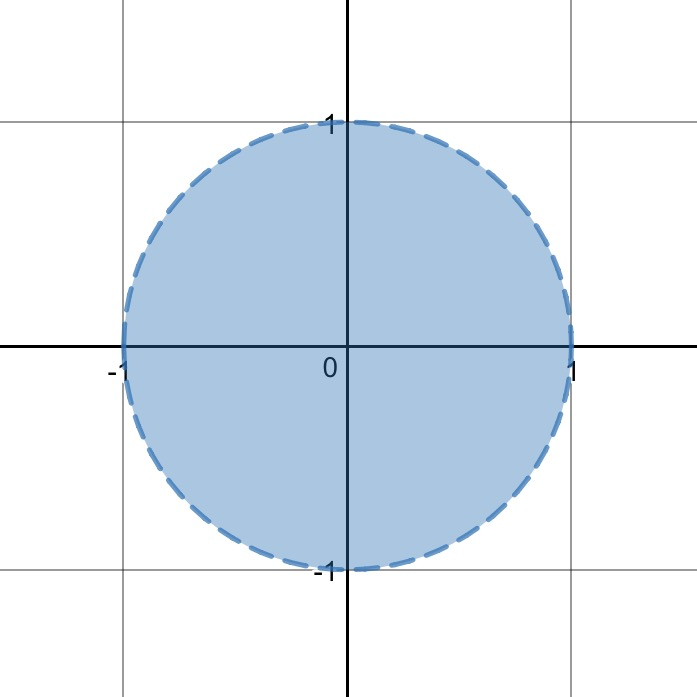
\includegraphics[scale=.125]{FullSizeRender}
\caption{The set $U$ in $\R^2$}
\end{figure}

Now, under $f$, every $n$-tuple in $\R^n$ maps either to itself, or to a corresponding $n$-tuple in the first orthant (or on its boundary); so the image of $U$ is $f(U)=U\cap I$, where $I$ denotes the closure of the first orthant.

\begin{figure}[h]
\centering
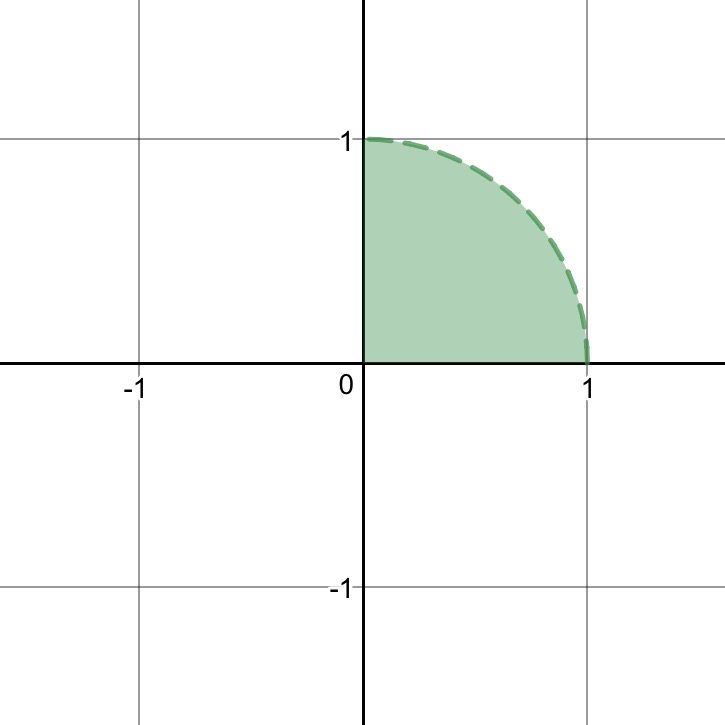
\includegraphics[scale=.125]{FullSizeRender1}
\caption{The set $f(U)$ in $\R^2$}
\end{figure}

The set $f(U)$ is not open; since the origin $\vec{0} \in f(U)$, but every $B(\vec{0},r)$ contains points in every orthant, so no open ball $B(\vec{0},r)$ is a subset of $f(U)$.

\begin{figure}[h]
\centering
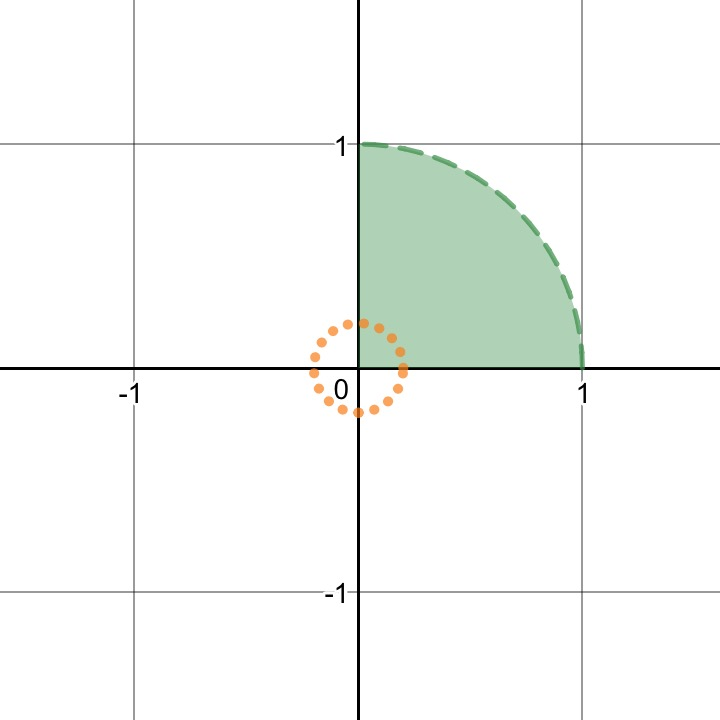
\includegraphics[scale=.125]{FullSizeRender2}
\caption{Every $B(\vec{0},r) \not\subset f(U)$}
\end{figure}

Therefore, (2) fails. Thus, (1) $\centernot\implies$ (2). 
\end{proof}
\end{example*}

\item Let $X = [0,\infty)$, and let $\T$ consist of $\emptyset$, $X$, and all sets of the form $(a,\infty)$ with $a\geq 0$. Show that $\T$ forms a topology on $X$. 

To prove that $\T$ forms a topology on $X$, it suffices to show the following: 
\begin{enumerate}[label=(\roman*)]
\item $\emptyset, X \in \T$ (This is true by assumption).
\item $\T$ is closed under arbitrary unions.
\item $\T$ is closed under finite intersections. 
\end{enumerate}

\begin{proof}\textbf{(ii)} Let $S$ be any subset of $\T$, and let $B = \{x:(x,\infty) \in S\}$. Then, since $\T$ contains all sets of the form $(a,\infty)$ with $a\geq 0$, it suffices to show that 
$$\bigcup S = (\inf(B),\infty).$$
$B$ is bounded below by $0$, so $\inf(B) \geq 0$ must exist.

$\subset$: For every $x \in B$ such that $x\neq \inf(B)$, $\inf(B) < x < \infty$. Therefore, every set in $S$ is a subset of $(\inf(B),\infty)$, so $\bigcup S \subset (\inf(B),\infty).$

$\supset$: Let $x \in (\inf(B),\infty)$; that is, $0 <\inf(B) < x$. If $\inf(B) \in B$, then $x \in (\inf(B),\infty) \subset \bigcup S$ and we are done. However, if $\inf(B) \not\in B$, then $\inf(B)$ must be a limit point of $B$, so every neighborhood of $\inf(B)$ contains an element of $B$ distinct from $\inf(B)$. Let $\delta = \frac{x-\inf(B)}{2}$, and consider the neighborhood $(\inf(B)-\delta, \inf(B)+\delta)$. Call $b$ the element of $B$ distinct from $\inf(B)$, and we find that $b < x$, so $x \in (b,\infty) \subset \bigcup S$.
\end{proof}

\begin{proof}\textbf{(iii)} Let $U, V \in \T$. In the trivial case where either set is empty, then $U \cap V = \emptyset$, and we are done. There is also another trivial case where $U=X$ and $V=X$. In this case, $U \cap V = X$, and we are done. So suppose $U$ and $V$ are nonempty sets, at least one of which is distinct from $X$; and let $u=\inf(U)$ and $v=\inf(V)$. Then, 
$$U \cap V= (\max(u,v),\infty),$$
which is a set of the form $(a,\infty)$, so $(\max(u,v),\infty) \in \T$.
\end{proof}

\item Let $X = [-1,1]$, and let $\T$ consist of all sets which either do not contain 0, or do contain the interval $(-1,1)$. Show that $\T$ forms a topology on $X$.

\begin{proof}Let $\T_U$ be the collection of all subsets of $X$ which do not contain 0, and let $\T_V$ be the collection of all subsets of $X$ which contain the interval (-1,1). 
\begin{enumerate}[label=(\roman*)]
\item $0 \not\in \emptyset$ and $(-1,1)\in X$, so $\emptyset, X \in \T$. 

\item Let $\{S_\alpha\}$ be an arbitrary collection of subsets of $\T$. If any of the sets in $\{S_\alpha\}$ contain $(-1,1)$, then $\bigcup_\alpha S_\alpha$ contains $(-1,1)$ as well. Otherwise, it consists only of sets which do not contain 0 (since they are all in $\T$), so $\bigcup_\alpha S_\alpha$ does not contain 0 either. Thererfore, $\T$ is closed under arbitrary unions.

\item Let $S_1, S_2$ be two sets in $\T$. If either set does not contain 0, then their intersection does not either. If neither set contains 0, then they both must contain $(-1,1)$, since they are both in $\T$. So, their intersection also contains $(-1,1)$. Therefore, $\T$ is closed under finite intersections.
\end{enumerate}
\end{proof}

\item Let $X$ be a nonempty set, with $p \in X$. Which of the following collections $\T$ form a topology on $X$? If it does, is it Hausdorff?
\begin{enumerate}
\item $\T$ consists of all subsets of $X$ which contain $p$, together with $\emptyset$. \\
\textbf{Claim: }$\T$ is a topology on $X$. 
\begin{proof}\mbox{}
\begin{enumerate}[label=(\roman*)]
\item $\emptyset, X \in \T$
\item Let $\{S_\alpha\}$ be an arbitrary collection of subsets of $\T$. If they all are empty, then their union is empty. Otherwise, at least one is nonempty, and so must contain $p$, so their union either contains $p$, or is empty. Thus, $\T$ is closed under arbitrary unions.
\item Let $S_1, S_2$ be two sets in $\T$. If either one is empty, then their intersection is empty. Otherwise, they both contain $p$, so their union either contains $p$, or is empty. Thus, $\T$ is closed under finite intersections.
\end{enumerate}
\end{proof}
\pagebreak
\textbf{Claim: }$(X, \T)$ is not Hausdorff. Following is a counterexample:
\begin{example*}
Consider $x,p \in X$. Since every set in $\T$ which is nonempty contains $p$, then there does not exist an open set which contains $x$ and not $p$. \qed
\end{example*}

\item $\T$ consists of all subsets of $X$ which do not contain $p$, together with $X$. \\
\textbf{Claim: }$\T$ is a topology on $X$. 
\begin{proof}\mbox{}
\begin{enumerate}[label=(\roman*)]
\item $\emptyset, X \in \T$
\item Let $\{S_\alpha\}$ be an arbitrary collection of subsets of $\T$. If any of them are the set $X$, then their union is $X$. Otherwise, none of them contain $p$, so their union either does not contain $p$, or is $X$. Thus, $\T$ is closed under arbitrary unions.
\item Let $S_1, S_2$ be two sets in $\T$. If both $S_1=X$ and $S_2=X$, then their intersection is $X$. Otherwise, at least one of them does not contain $p$, so their union either does not contain $p$, or is empty. Thus, $\T$ is closed under finite intersections.
\end{enumerate}
\end{proof}
\textbf{Claim: }$(X, \T)$ is not Hausdorff. Following is a counterexample:
\begin{example*}
Consider $x,p \in X$. Since the only set in $\T$ which contains $p$ is $X$, then there do not exist any open set which are disjoint from the one containing $p$. \qed
\end{example*}
\end{enumerate}

\item Let $(X, \T)$ be a topological space, with $q \not\in X$. Is $\T^*=\{U\cup \{q\}:U\in \T\}\cup\{0\}$ a topology on $X\cup\{q\}$? If so, is it Hausdorff?\\
\textbf{Claim: }$\T$ is a topology on $X$, but is not Hausdorff.
\begin{proof}First, note that $\T^*$ consists only of subsets of $X\cup \{q\}$ which contain $q$, together with $\emptyset$. This topological space has the same form as that of problem 4(a). So, by the same reasons given in problem 4(a), $\T$ is a topology on $X$, but is not Hausdorff.
\end{proof} 

\end{enumerate}

\end{document}